\documentclass[10pt,fleqn,xcolor=dvipsnames]{beamer}
\beamertemplatenavigationsymbolsempty
\usetheme{Boadilla}
\DeclareGraphicsExtensions{.jpg,.eps,.png,.pdf,.mps,.gif}
\usepackage[latin1]{inputenc}
\usepackage[T1]{fontenc}
\usepackage[english]{babel}
\usepackage{pgf,pgfarrows,pgfnodes,pgfautomata,pgfheaps}
\usepackage{amsmath}
\usepackage{amsfonts}
\usepackage{graphicx}
\usepackage{color}
\usepackage{lmodern}
\usepackage[3D]{movie15}
%\usepackage{algorithm}
%\usepackage{algpseudocode}
\usepackage{url}
\usepackage{placeins}
\usepackage{listings}
\lstset{language=bash}
\colorlet{grey}{gray!40}
\definecolor{PG}{rgb}{0.0, 0.27, 0.13}
%%%%%%%%%%%%%%%%%%%%%%%%%%%%%%%%%%%%%%%%%%%%%%%%%%%%%%%%%%%%%%%%%%%%%%%%%%%%%%%%%%%%%%%
% title page definition %%%%%%%%%%%%%%%%%%%%%%%%%%%%%%%%%%%%%%%%%%%%%%%%%%%%%%%%%%%%%%%
%%%%%%%%%%%%%%%%%%%%%%%%%%%%%%%%%%%%%%%%%%%%%%%%%%%%%%%%%%%%%%%%%%%%%%%%%%%%%%%%%%%%%%%
\setbeamercovered{dynamic}
\setbeamerfont{author}{family=\rmfamily}
\author[M. Beccuti and R. J.P. Bonnal]{\large{\textbf{M. Beccuti and R. J. P. Bonnal}}\\[15pt]\emph{Universit\`{a} degli Studi di Torino, Istituto Nazionale di Genetica Molecolare  Romeo ed Enrica Invernizzi \\[5pt]} \textbf{ELIXIR-IIB Training Platform}}
\title[ELIXIR-IIB Training Platform]{\Large{\textbf{Docker and Reproducibility}}}
%\institute{\normalsize{} \\
\date[13,14 June 2019]{13,14 June 2019}
\titlegraphic{
\includegraphics[height=2cm]{Figure/LogoTorino}}

% table of contents depth
\setcounter{tocdepth}{1}
\begin{document}
\usebackgroundtemplate{
\includegraphics[width=140mm]{Figure/BackgroundTorino}}
\setcounter{tocdepth}{5}
%#Frame 1 title
\frame[plain]{\titlepage}


\frame{
\frametitle{Outline}  \vspace{0.3cm}
\begin{block}{Training day aims:}
\begin{itemize}
  \item Understanding Docker Volumes and Storage
  \item Dockerfile and best practices; 
  \item Deploy a private registry;
  \item ...
\end{itemize}    
\end{block}
\vspace{0.5cm}
\begin{enumerate}
  \item A short introduction  recalling the concepts described in the first day\vspace{0.2cm}
  \begin{itemize}
    \item ...; \vspace{0.2cm}
    \item ...; \vspace{0.2cm}
  \end{itemize}

  \item ...; \vspace{0.2cm}
  \item ...;\vspace{0.2cm}
  \item ....;\vspace{0.2cm}
  \item Deploy services on a cluster using docker swarm.
\end{enumerate}
}

\frame{
\frametitle {}
\vspace{2cm}
\centerline{\Huge \color{NavyBlue} \textbf{\emph{Volumes}}}
\vspace{0.5cm}
}
\frame{
\frametitle{Data in Docker}
We are in a containerized world.\\
Everything is separated.\\
How do we share/access data ?\\
}

\frame{
\frametitle{Data in Docker: Goals}
\begin{itemize}
\item How Docker manages data ?
\item Use different type of data storage
\end{itemize}
}

\frame{
\frametitle{Data in Docker}
Docker has 3 options
\begin{itemize}
\item Volumes
\item Bind Mounts
\item tmpfs mount
\end{itemize}
}


\frame{
\frametitle{Data in Docker}
Docker and data
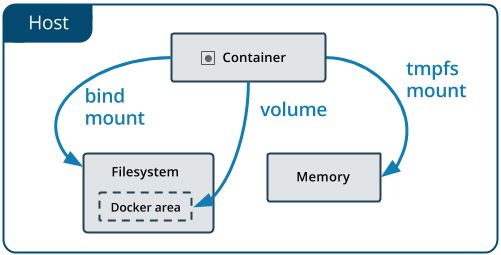
\includegraphics[width=0.50\columnwidth]{./Figure/docker-080-054}
}

\frame{
\frametitle{Data in Docker}
\framesubtitle{Volumes}
\begin{itemize}
\item Managed directly by Docker
\item Saved in \lstinline!/var/lib/docker/volumes/! on the host
\item System processes can not access data outside Docker
\item Recommended by Docker to store data in Docker
\end{itemize}
}

\frame{
\frametitle{Data in Docker}
\framesubtitle{Volumes}

\begin{itemize}
\item User can create its own volumes or instruct Docker to create them when required by the containers or services
\item The container see the volume as a directory and the user define the name
\item Docker guarantees isolation from the host machine
\item A volume can be mounted by many containers at the same time
\end{itemize}
}

\frame{
\frametitle{Data in Docker}
\framesubtitle{Volumes}
\begin{itemize}
\item If not used it is not destroyed, the user must remove the volume explicitly
\item The user can name a volume or Docker create a random name automatically
\item A volume can be an \it{object} in the cloud, the user must use a proper \it{driver}
\item Avoid to increase the size of the container
\end{itemize}
}

\frame{
\frametitle{Data in Docker}
\framesubtitle{Bind mounts}

\begin{itemize}
\item Managed directly by the host OS
\item Saved in  \emph{\color{PineGreen} /in/your/path/} on the host OS
\item System processes or Docker containers can access to the data
\item It is possible to override important files or directory on the host OS
\end{itemize}

}

\frame{
\frametitle{Data in Docker}
\framesubtitle{Bind mounts}

\begin{itemize}
\item Files and directory from the host are mounted inside the container at runtime
\item Require the target's full path on the host machine
\item On demand creation inside the container
\item Very performant
\item Rely on the host filesystem
\item From inside the contianer the user has full access to the filesystem: read/write
\item Read/Write from outside the Docker container
\end{itemize}
}

\frame{
\frametitle{Data in Docker}

Expose a \it{Volume} or \it{Bind Mount} into the container

 \emph{\color{PineGreen} --volume | -v}

Docker infers if it is a \it{Volume} or a \it{Bind Mount} from the command line
}

\frame{
\frametitle{Data in Docker}

In memory storage

 \emph{\color{PineGreen} --tmpfs}

This is useful for ephemeral storage
}

\begin{frame}[fragile]
\frametitle{Data in Docker}
\framesubtitle{When use What}

\begin{itemize}
\item \textit{Volume}
  \begin{itemize}
  \item Sharing data among containers
  \item The host lacks a directory structure
  \item Data can not be stored locally (cloud)
  \end{itemize}
\item \textit{Bind mount}
  \begin{itemize}
  \item Sharing configuration to containers
  \item Sharing source code and build products
  \item Stable directory and file structures shared w/ containers
  \end{itemize}
\end{itemize}
\end{frame}

\begin{frame}[fragile]
\frametitle{Data in Docker}
\framesubtitle{CLI}

\begin{lstlisting}
 docker volume

Commands:
  create   Create a volume
  inspect  Display detailed information on one or more
           volumes
  ls       List volumes
  prune    Remove all unused volumes
  rm       Remove one or more volumes
\end{lstlisting}
\end{frame}


\begin{frame}[fragile]
\frametitle{Data in Docker}
\framesubtitle{Create a volume}

\begin{lstlisting}
$ docker volume create edr19-storage

edr19-storage
\end{lstlisting}
\end{frame}

\begin{frame}[fragile]
\frametitle{Data in Docker}
\framesubtitle{List volumes}


\begin{lstlisting}
$ docker volume ls

DRIVER    VOLUME NAME
local     edr19-storage
\end{lstlisting}
\end{frame}

\begin{frame}[fragile]
\frametitle{Data in Docker}
\framesubtitle{Inspecting a volume}
\begin{lstlisting}[breaklines=true]
$ docker volume inspect edr19-storage

[{
  "CreatedAt": "2019-05-20T18:38+00:00",
  "Driver": "local",
  "Labels": {},
  "Mountpoint": "/var/lib/docker/volumes/edr19-storage/_data",
  "Name": "edr19-storage",
  "Options": {},
  "Scope": "local"
  }]
\end{lstlisting}

\end{frame}

\begin{frame}[fragile]
\frametitle{Data in Docker}
\framesubtitle{Use a volume}

Run a container with Ubuntu 18.04 and create a file with something inside
\begin{lstlisting}
$ docker run --rm \
             -v edr19-storage:/data \
             -it ubuntu:18.04 /bin/bash 
$ echo $RANDOM > /data/seed
$ exit
\end{lstlisting}

After closing the container data are stored an can be accessed
by another container

\begin{lstlisting}
$ docker run --rm \
             -v edr19-storage:/data \
             -it ubuntu:18.04 /bin/bash \
             -c "cat /data/seed"
\end{lstlisting}
\end{frame}

\begin{frame}[fragile]
\frametitle{Data in Docker}
\framesubtitle{Mount points}

Load your own directory inside the container

\begin{lstlisting}
$ docker run -v /opt:/host/opt \
             --name edr19 \
             --rm \
             -it ubuntu:18.04 /bin/bash
\end{lstlisting}
\end{frame}

\begin{frame}[fragile]
\frametitle{Data in Docker}
\framesubtitle{Mount points}

Load your own directory inside the container

\begin{lstlisting}
$ docker run -v /opt:/host/opt \
             --name edr19 \
	      --rm \
            -it ubuntu:18.04 /bin/bash

\end{lstlisting}

\it{Docker does not like relative path}
\end{frame}

\begin{frame}[fragile]
\frametitle{Data in Docker}
\framesubtitle{Volumes and Mount points}

Combine volumes and mount points in a single instance

\begin{lstlisting}
$ docker run -v /opt:/host/opt \
             -v edr19-storage:/data \
             --name edr19 \
             --rm \
             -it ubuntu:18.04 /bin/bash
\end{lstlisting}
\end{frame}

\begin{frame}[fragile]
\frametitle{Data in Docker}
\framesubtitle{Share data w/ containers}


\begin{lstlisting}
$ docker run -v /opt:/host/opt \
             -v edr19-storage:/data \
             --name edr19 \
             --rm \
             -it ubuntu:18.04 /bin/bash

\end{lstlisting}
Another container can access to the data at the same time
\begin{lstlisting}
$ docker run --volumes-from edr19 \
             --name backup \
             --rm \
             -it ubuntu:18.04 /bin/bash
\end{lstlisting}
\it{You may notice some lag in updating data, it depends on the underlying Docker filesystem}
\end{frame}

\begin{frame}[fragile]
\frametitle{Data in Docker}
\framesubtitle{Share data w/ containers}

\scriptsize
\begin{lstlisting}
$ docker run -v /opt:/host/opt \
             -v edr19-storage:/data \
             --name edr19 \
             --rm \
             -it ubuntu:18.04 /bin/bash
\end{lstlisting}
\normalsize
Another container can access to the data and perform a backup automatically
\scriptsize
\begin{lstlisting}
$ docker run --volumes-from edr19 \
             --name backup \
            --rm \
            -it ubuntu:18.04 \
            tar vcz /host/opt/backup.tar.gz /data
\end{lstlisting}
\normalsize
\it{You may notice some lag in updating data, it depends on the underlying Docker filesystem}
\end{frame}

\begin{frame}[fragile]
\frametitle{Data in Docker}
\framesubtitle{Volumes on the fly}

When needed you can even create a Volume at runtime w/o using the explicit \lstinline{create} command. 

\begin{lstlisting}
$ docker run -v bioinfo:/reads \
             -v /opt:/host/opt \
             -v edr19-storage:/data \
             --name edr19 \
             --rm \
             -it ubuntu:18.04 /bin/bash
\end{lstlisting}
\end{frame}

\begin{frame}[fragile]
\frametitle{Data in Docker}
\framesubtitle{Volumes on the fly}

When needed you can even create a Volume at runtime w/o using the explicit \lstinline{create} command. 

\begin{lstlisting}
$ docker volume ls

DRIVER    VOLUME NAME
local     edr19-storage
local     bioinfo
\end{lstlisting}
\end{frame}

\begin{frame}[fragile]
\frametitle{Data in Docker}
\framesubtitle{Anonymous Volumes} 

When needed you can even create a Volume at runtime w/o using the explicit \lstinline{create} command. 

\begin{lstlisting}
$ docker run -v /anonymous \
             -v bioinfo:/reads \
             -v /opt:/host/opt \
             -v edr19-storage:/data \
             --name edr19 \
             --rm \
             -it ubuntu:18.04 /bin/bash
\end{lstlisting}
\end{frame}

\begin{frame}[fragile]
\frametitle{Data in Docker}
\framesubtitle{Anonymous Volumes}

When needed you can even create a Volume at runtime w/o using the explicit \lstinline{create} command. 

\begin{lstlisting}
$ docker volume ls

DRIVER    VOLUME NAME
local     edr19-storage
local     bioinfo
\end{lstlisting}

\it{Once exited from the container, there is no evidence about the anonymous container}
\end{frame}

\begin{frame}[fragile]
\frametitle{Data in Docker}
\framesubtitle{Anonymous Volumes}

w/o \lstinline{--rm}

When needed you can even create a Volume at runtime w/o using the explicit \lstinline!create! command. 


\begin{lstlisting}
$ docker run -v /anonymous \
             -v bioinfo:/reads \
             -v /opt:/host/opt \
             -v edr19-storage:/data \
             --name edr19 \
             -it ubuntu:18.04 /bin/bash
\end{lstlisting}
\end{frame}

\begin{frame}[fragile]
\frametitle{Data in Docker}
\framesubtitle{Anonymous Volumes}
 w/o \lstinline{--rm}

When needed you can even create a Volume at runtime w/o using the explicit \lstinline{create} command. 


\begin{lstlisting}
$ docker volume ls

DRIVER    VOLUME NAME
local     edr19-storage
local     bioinfo
local     8a76g20jc0gcbgf3952gbdnihd253r801skala7898y...
\end{lstlisting}
\end{frame}

\begin{frame}[fragile]
\frametitle{Data in Docker}
\framesubtitle{Tech notes}

Docker \it{volumes}, \it{images}, \it{container} are capped to a defaul value which is configured at daemon level usually around \texttt{10 GB}

\begin{lstlisting}
dm.basesize
\end{lstlisting}
\end{frame}

\frame{
\frametitle{Data in Docker}
\framesubtitle{Tech notes}

The \lstinline{dm.basesize} can be increased but the Docker's daemon must be restared.
}

\begin{frame}[fragile]
\frametitle{Data in Docker}
\framesubtitle{Tech notes}

The user can run the daemon by hand 
\begin{lstlisting}
$ sudo dockerd --storage-opt dm.basesie=50G
\end{lstlisting}
\end{frame}

\frame{
\frametitle{Data in Docker}
\framesubtitle{Tech notes}

The user can increase the size but never decrease it.

If the user specifes a value which is lower than the minimum size of \it{volumes}, \it{images}, \it{containers} Docker will complain with errors.
}

\begin{frame}[fragile]
\frametitle{Data in Docker}
\framesubtitle{Tech notes}

Usually everything works fine, but may happend that Docker' system dir should be wiped out
\begin{lstlisting}
$ sudo service docker stop

$ sudo rm -rf /var/lib/docker
\end{lstlisting}
\end{frame}

\frame{
\frametitle {}
\vspace{2cm}
\centerline{\Huge \color{NavyBlue} \textbf{\emph{Storage}}}
\vspace{0.5cm}
}
\frame{
\frametitle{Docker Storage}
Every piece of data in Docker is a layer.
\vspace{0.4cm}
Layers can be (are) resued when possible.
\vspace{0.4cm}
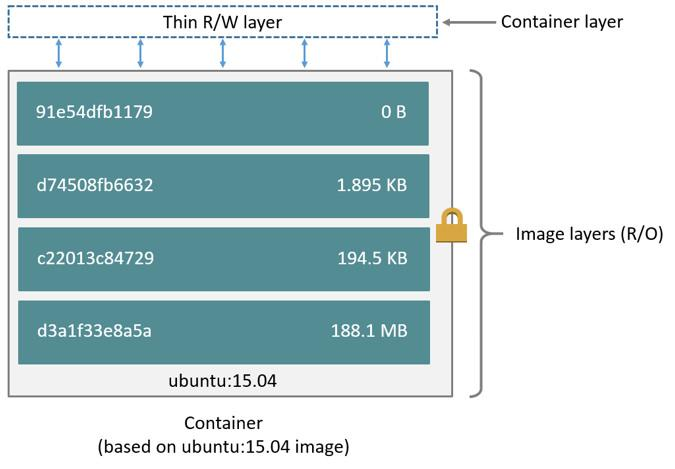
\includegraphics[width=0.50\columnwidth]{./Figure/docker-064-046}
}

\frame{
\frametitle{Docker Storage}
\framesubtitle{Layers}
Layers are a sort of snapshots of a filesystem
\vspace{0.4cm}
Usually are in readonly mode
\vspace{0.4cm}
To every new container a \it{Thin} r/w layer is created. In this layer the container can store its own data.
}

\begin{frame}[fragile]
\frametitle{Docker Storage}
\framesubtitle{Layers}
\begin{columns}
\begin{column}{.65\textwidth}
\begin{lstlisting}
FROM ubuntu:15.04
COPY ./app
RUN make /app
CMD python /app/app.py
\end{lstlisting}
\end{column}
\begin{column}{.35\textwidth}
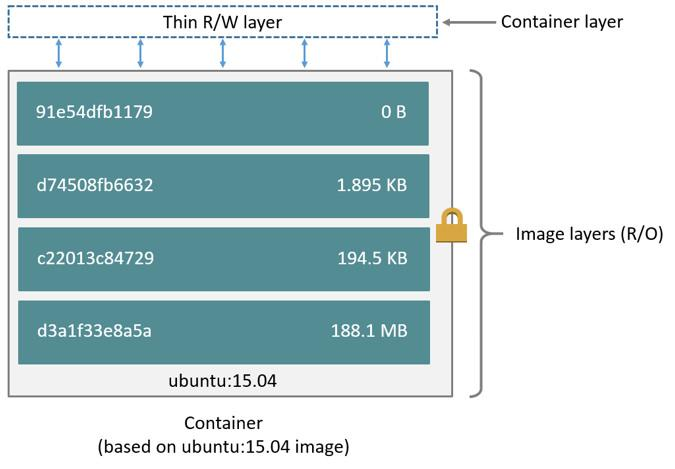
\includegraphics[width=1\columnwidth]{./Figure/docker-064-046}
\end{column}
\end{columns}
\end{frame}

\begin{frame}[fragile]
\frametitle{Docker Storage}
\framesubtitle{Pull and Storage}
\begin{lstlisting}
$ docker pull ubuntu:15.04

15.04: Pulling from library/ubuntu
1ba8ac955b97: Pull complete
f157c4e5ede7: Pull complete
0b7e98f84c4c: Pull complete
a3ed95caeb02: Pull complete
Digest: sha256:5e279a9df07990286cce22e1b0f5b049062
	9ca6d187698746ae5e28e604a640e
Status: Downloaded newer image for ubuntu:15.04
\end{lstlisting}
\end{frame}

\begin{frame}[fragile]
\frametitle{Docker Storage}
\framesubtitle{Pull and Storage}
\begin{lstlisting}
$ docker pull ubuntu:18.04
18.04: Pulling from library/ubuntu
124c757242f8: Pull complete
9d866f8bde2a: Pull complete
fa3f2f277e67: Pull complete
398d32b153e8: Pull complete
afde35469481: Pull complete
Digest: sha256:de774a3145f7ca4f0bd144c7d4ffb2931e0
	6634f11529653b23eba85aef8e378
Status: Downloaded newer image for ubuntu:18.04
\end{lstlisting}
\end{frame}


\begin{frame}[fragile]
\frametitle{Docker Storage}
\framesubtitle{Pull and Storage}
\begin{lstlisting}
$ docker images -f reference='ubuntu'

REPOSITORY   TAG     IMAGE ID      CREATED      SIZE
ubuntu       18.04   cd6d8154f1e1  2 weeks ago  84.1MB
ubuntu       16.04   2dc7f0e4fc33  2 years ago  122MB
ubuntu       14.04   54060fb55e83  3 years ago  188MB
\end{lstlisting}
\end{frame}

\begin{frame}[fragile]
\frametitle{Docker Storage}
\framesubtitle{Pull and Storage}
\begin{lstlisting}
$ sudo find /var/lib/docker -name cd6d81*

/var/lib/docker/image/aufs/imagedb/content/sha256/
	cd6d8154f1e16e38493c3c2798977c5e142be5e5d41403
	ca89883840c6d51762

\end{lstlisting}
\end{frame}

\begin{frame}
\frametitle{Docker Storage}
\framesubtitle{Drivers}
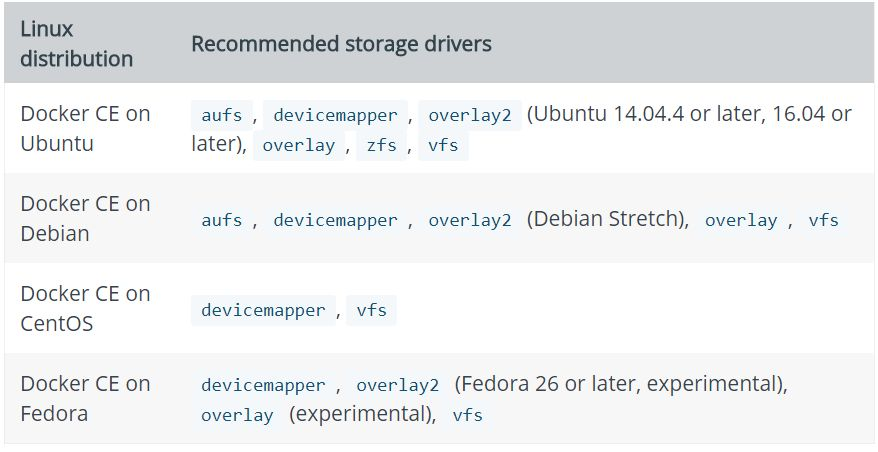
\includegraphics[width=1.0\columnwidth]{./Figure/docker-070-052}
\end{frame}

\begin{frame}
\frametitle{Docker Storage}
\framesubtitle{Drivers}
\begin{itemize}
\item aufs, overlay, overlay2: work at file level, memory efficient but layers can grow and become inefficient with high I/O
\item devicemapper,btrfs, zfs: block-level storage, works with write-heavy I/O
\item btrfs, zfs: require a lot of memory
\item zfs: is a good choice for high-density workloads such as PaaS
\item overlay: works better with many layers and small files compared to overlay2
\end{itemize}
\end{frame}


\begin{frame}
\frametitle{Docker Storage}
\framesubtitle{Drivers}

How to choose the driver:
\begin{itemize}
\item Perform tests based on your hardware with your sysadmin
\item Check the stability of the driver and decide your stability policy
\item If you have an expertise in house use it
\item Some drivers works best on some Linux distro
\item Perform tests on real workloads
\end{itemize}
\end{frame}

\begin{frame}
\frametitle{Docker Storage}
\framesubtitle{Drivers}
\it{!!! WARING !!!}
\vspace{0.4cm}
You can not mix drivers
\vspace{0.4cm}
Each driver has its set of images and containers
\vspace{0.4cm}
Migration is not possible
\end{frame}


\begin{frame}
\frametitle{Docker Storage}
\framesubtitle{Layers}
Layers are a sort of snapshots of a filesystem
\vspace{0.4cm}
Usually are in readonly mode
\vspace{0.4cm}
To every new container a \it{Thin} r/w layer is created. In this layer the container can store its own data.
\end{frame}

\begin{frame}
\frametitle{Docker Storage}
\framesubtitle{Thin layers}
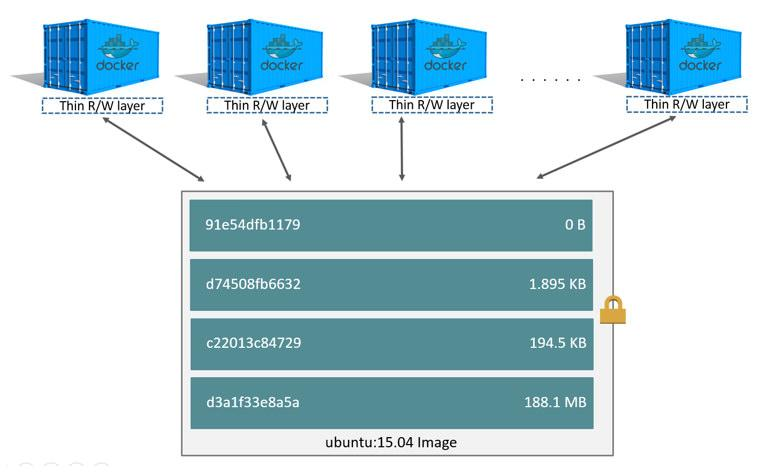
\includegraphics[width=0.5\columnwidth]{./Figure/docker-065-047}
\end{frame}


\begin{frame}
\frametitle{Docker Storage}
\framesubtitle{Thin layers and Data}
A writable container layer is created every time a container starts and it is where data are stored.
\vspace{0.4cm}
When a container is not running:
\begin{itemize}
\item Data does not persist
\item Sharing data with other container is very very ... very complicated
\item Your host machine own the writable layer, moving the layer is not that simple
\item Not the best option for high I/O, layers can be asynchronous 
\end{itemize}
\end{frame}

\begin{frame}[fragile]
\frametitle{Docker Storage}
\framesubtitle{Thin layers}
\begin{lstlisting}
$ docker run -dit --name my_container_1
           acme/my-final-image:1.0 bash

c36785c423ec7e0422b2af7364a7ba4da6146cbba7981a0951
	fcc3fa0430c409


$ docker run -dit --name my_container_2 
           acme/my-final-image:1.0 bash
		   
dcad7101795e4206e637d9358a818e5c32e13b349e62b00bf0
	5cd5a4343ea513

...
\end{lstlisting}
\end{frame}

\begin{frame}[fragile]
\frametitle{Docker Storage}
\framesubtitle{Thin layers, where are }
\begin{lstlisting}
$ sudo du -shL /var/lib/docker/containers/*
32K /var/lib/docker/containers/1a174fc216cccf18ec7
	d4fe14e008e30130b11ede0f0f94a87982e310cf2e765
32K /var/lib/docker/containers/1e7264576d78a3134fb
	af7829bc24b1d96017cf2bc046b7cd8b08b5775c33d0c
32K /var/lib/docker/containers/38fa94212a419a082e6
	a6b87a8e2ec4a44dd327d7069b85892a707e3fc818544
32K /var/lib/docker/containers/c36785c423ec7e0422b
	2af7364a7ba4da6146cbba7981a0951fcc3fa0430c409
32K /var/lib/docker/containers/dcad7101795e4206e63
	7d9358a818e5c32e13b349e62b00bf05cd5a4343ea513 
\end{lstlisting}
\end{frame}

\begin{frame}[fragile]
\frametitle{Docker Storage}
\framesubtitle{Container and Size}
Running a plain Ubuntu 18.04
\vspace{0.4cm}
\begin{lstlisting}
$ docker run ubuntu -it ubuntu:18.04 bash
\end{lstlisting}
\vspace{0.4cm}
\it{Note} detach from the container using \lstinline!Ctrl-P! + \lstinline!Ctrl-Q!
\end{frame}

\begin{frame}[fragile]
\frametitle{Docker Storage}
\framesubtitle{Container and Size}
\begin{lstlisting}
$ docker ps -s


| CONTAINER ID | IMAGE        | SIZE                |

| 0e7438744a0a | ubuntu:18.04 | 0B (virtual 84.1MB) |
\end{lstlisting}
\end{frame}

\begin{frame}[fragile]
\frametitle{Docker Storage}
\framesubtitle{Container and Size}
Updating the \lstinline!apt! database
\vspace{0.4cm}
\begin{lstlisting}
$ docker attach 0e74

$ apt update


| CONTAINER ID | IMAGE        | SIZE                   |

| 0e7438744a0a | ubuntu:18.04 | 41.7MB (virtual 126MB) |
\end{lstlisting}
\end{frame}

\begin{frame}[fragile]
\frametitle{Docker Storage}
\framesubtitle{Container and Size}
Upgrading the \lstinline!apt! database
\vspace{0.4cm}
\begin{lstlisting}
$ apt upgrade


| CONTAINER ID | IMAGE        | SIZE                   |

| 0e7438744a0a | ubuntu:18.04 | 42.6MB (virtual 127MB) |
\end{lstlisting}
\end{frame}

\begin{frame}[fragile]
\frametitle{Docker Storage}
\framesubtitle{Container and Size}
Installing \lstinline!wget!
\vspace{0.4cm}
\begin{lstlisting}
$ apt install wget


| CONTAINER ID | IMAGE        | SIZE                   |

| 0e7438744a0a | ubuntu:18.04 | 49.1MB (virtual 133MB) |
\end{lstlisting}
\end{frame}




\frame{
\frametitle {}
\vspace{2cm}
\centerline{\Huge \color{NavyBlue} \textbf{\emph{Dockerfile}}}
\vspace{0.5cm}
}
\begin{frame}
\frametitle{Dockefile}

A docker can be created by hand

\begin{itemize}
\item pull an image
\item star a container
\item modify the container
\item commit the changes 
\end{itemize}

this is more or less the process for creating a reusable container \textit{an Image}
\end{frame}

\begin{frame}
\frametitle{Dockerfile}

By \textit{hand} is good for practicing or testing but is very bad for 
\begin{itemize}
\item reproducibility
\item automation
\item dependencies
\end{itemize}
\end{frame}

\begin{frame}
\frametitle{Dockerfile}

By \textit{hand} is good for practicing or testing but is very bad for 

\begin{itemize}
\item \textit{reproducibility}: lost the history of the commands that create the final image
\item automation
\item dependencies
\end{itemize}
\end{frame}

\begin{frame}
\frametitle{Dockerfile}

By \textit{hand} is good for practicing or testing but is very bad for 

\begin{itemize}
\item reproducibility
\item \textit{automation}: images are lost because some disaster and eveything was on a local machine
\item dependencies
\end{itemize}
\end{frame}

\begin{frame}
\frametitle{Dockerfile}

By \textit{hand} is good for practicing or testing but is very bad for 

\begin{itemize}
\item reproducibility
\item automation
\item \textit{dependencies}: images are build from other images and something must be changed in the original image
\end{itemize}
\end{frame}

\begin{frame}
\frametitle{Dockerfile}
\framesubtitle{what is it?}

A simple text files with all the instructions for

\begin{itemize}
\item start (PULL) from a (public) Linux distribution
\item install software
\item configure the installation
\item configure the container for running automatically
\end{itemize}
\end{frame}

\begin{frame}[fragile]
\frametitle{Dockerfile}
\framesubtitle{what is it?}

The most minimal \lstinline!Dockerfile!
\begin{lstlisting}
FROM ubuntu:18.04
\end{lstlisting}

\textit{Note} by convention \lstinline!Dockerfile! is the name to use for the file containing the instructions.
\end{frame}


\begin{frame}[fragile]
\frametitle{Dockerfile}
\framesubtitle{How to use it}

A \lstinline!Dockerfile! can be used for building a new image

\begin{lstlisting}
 $ docker build -t origin .
 Sending build context to Docker daemon  2.048kB
 Step 1/1 : FROM ubuntu:18.04
  ---> cd6d8154f1e1
  Successfully built cd6d8154f1e1
  Successfully tagged origin:latest
\end{lstlisting}

A new image is created with the \lstinline!sha256! \lstinline!cd6d8154f1e1! called \lstinline!origin! and the version, in this case by default \lstinline!Docker! assign the tag \lstinline!latest!
\end{frame}

\begin{frame}[fragile]
\frametitle{Dockerfile}
\framesubtitle{FROM}

Start from a Linux distribution or previous installations/images

\begin{lstlisting}
FROM <image> [AS <name>]

FROM <image>[:<tag>] [AS <name>]

FROM <image>[@<digest>] [AS <name>]
\end{lstlisting}
\end{frame}

\begin{frame}[fragile]
\frametitle{Dockerfile}
\framesubtitle{LABEL}

Metadata are useful in order to describe the image, making it more consumable by others

\lstinline!LABEL <key>=<value> <key>=<value> <key>=<value> ...!

\begin{lstlisting}
LABEL org.ingm.group="Your Boss name"
LABEL maintainer="Bonnal Raoul J.P. <bonnal@ingm.org>"
LABEL project="Elixir Test"
LABEL description="Dockerfile example \
with multiple lines."
LABEL version="1.2"
 
LABEL maintainer=''bonnal@ingm.org''
\end{lstlisting}

User is free to use any kind of \lstinline!key=val! convention but the \textit{reverse DNS} notation.
\end{frame}

\begin{frame}[fragile]
\frametitle{Dockerfile}
\framesubtitle{ENV}

Environment variables can be set inside the container

\begin{lstlisting}
ENV <key> <value>
ENV <key>=<value> ...
\end{lstlisting}

\begin{lstlisting}[breaklines=true]
ENV software="samtools" description=A\ great\ piece\ of\ software
    author=someone
\end{lstlisting}	
and
	
\begin{lstlisting}
ENV software samtools
ENV description A great piece of software
ENV author someone
\end{lstlisting}

these variable are available during the building process and when the container is running
\end{frame}

\begin{frame}[fragile]
\frametitle{Dockerfile}
\framesubtitle{WORKDIR}

Sets the working directory for the following \textit{instructions}

\begin{lstlisting}
ENV MYSUBDIR mytmp
RUN mkdir /opt/$MYSUBDIR
WORKDIR /opt/$MYSUBDIR
RUN pwd
\end{lstlisting}

Works for \lstinline!RUN!, \lstinline!CMD!, \lstinline!ENTRYPOINT!, \lstinline!COPY! and \lstinline!ADD!
\end{frame}

\begin{frame}[fragile]
\frametitle{Dockerfile}
\framesubtitle{injecting files}

To fully customize the image, external files can be included. To achieve this \textit{Docker} provides two different tools

\begin{itemize}
\item \lstinline!ADD!
\item \lstinline!COPY!
\end{itemize}
\end{frame}

\begin{frame}[fragile]
\frametitle{Dockerfile}
\framesubtitle{ADD}

\begin{lstlisting}
ADD [--chown=<user>:<group>] <src>... <dest>
ADD [--chown=<user>:<group>] ["<src>",... "<dest>"]
\end{lstlisting}
\begin{itemize}
\item Digest URLs, download
\item Unpack archives (identity, gzip, bzip2 or xz)
\item Does not perform authentication
\item At every build it is re excuted
\end{itemize}
\end{frame}

\begin{frame}[fragile]
\frametitle{Dockerfile}
\framesubtitle{COPY}

\begin{lstlisting}
COPY [--chown=<user>:<group>] <src>... <dest>
COPY [--chown=<user>:<group>] ["<src>",... "<dest>"]
\end{lstlisting}

\begin{itemize}
\item Relative path outside of context does not work
\item Works only with local files or directory
\item Can copy files from source location to a previous build stage \lstinline!FROM!
\item NO URLs
\item NO auto unpacking
\end{itemize}
\end{frame}

\begin{frame}[fragile]
\frametitle{Dockerfile}
\framesubtitle{SHELL}

When commands must be run with a different shell

\begin{lstlisting}
SHELL ["executable", "parameters"]
\end{lstlisting}
\end{frame}

\begin{frame}[fragile]
\frametitle{Dockerfile}
\framesubtitle{USER}

Set the USER to use during when the containers run.
It also set the user for \lstinline!RUN!, \lstinline!CMD!, \lstinline!ENTRYPOINT! following the declaration of \lstinline!USER!

\begin{lstlisting}
USER <user>[:<group>]
USER <UID>[:<GID>]
\end{lstlisting}
\end{frame}

\begin{frame}[fragile]
\frametitle{Dockerfile}
\framesubtitle{RUN}

To customise the installation the user must execute commands.

The commands are run inside a default shell \lstinline!/bin/sh -c!

Use the \lstinline!SHELL! clause to change the shell for the following \lstinline!Dockerfile!

When a \lstinline!RUN! succeed Docker will write a layer.
\end{frame}

\begin{frame}[fragile]
\frametitle{Dockerfile}
\framesubtitle{RUN}

\lstinline!RUN! have two forms:

\begin{lstlisting}
RUN apt-get update
\end{lstlisting}

or use a more explicit form where parameters are passed in a sort of \lstinline!JSON! notation

\begin{lstlisting}
RUN ["apt-get", "update"]
\end{lstlisting}

The JSON form does not create a shell for the command, so variable can not be substituted. To use the shell substitution call the shell first.
\end{frame}

\begin{frame}[fragile]
\frametitle{Dockerfile}
\framesubtitle{RUN}

\begin{lstlisting}
RUN apt-get install -y wget git python3.6
\end{lstlisting}

A \lstinline!RUN! command can span multiple lines


\begin{lstlisting}
RUN apt-get install -y wget \
                       git \
				  python3.6
\end{lstlisting}
\end{frame}

\begin{frame}[fragile]
\frametitle{Dockerfile}
\framesubtitle{RUN}

A \lstinline!RUN! command can be made by multiple commands

\begin{lstlisting}
RUN comamnd1 && command2
\end{lstlisting}

The \lstinline!RUN! will pass and create a layer only if it succeed. Otherwise, Docker will report the original error.
\end{frame}

\begin{frame}[fragile]
\frametitle{Dockerfile}
\framesubtitle{RUN}

Combining commands and spanning the commands on multiple lines helps in readability and building complex configurations.

\begin{lstlisting}
RUN apt-get update &&\
    apt-get install -y wget 
\end{lstlisting}
\end{frame}

\begin{frame}[fragile]
\frametitle{Dockerfile}
\framesubtitle{RUN}

Combining commands and spanning the commands on multiple lines helps in readability and building complex configurations.

\begin{lstlisting}
RUN apt-get update &&\
    apt-get install -y wget \
	                   git \
	                   python3.6
\end{lstlisting}
\end{frame}

\begin{frame}[fragile]
\frametitle{Dockerfile}
\framesubtitle{ENTRYPOINT}
Defines a container that runs as an executable

Forms:

\begin{itemize}
\item \textit{exec}: preferred \lstinline!ENTRYPOINT ["executable", "param1", "param2"]!

\item \textit{shell}:  \lstinline!ENTRYPOINT command param1 param2!
\end{itemize}
\end{frame}


\begin{frame}[fragile]
\frametitle{Dockerfile}
\framesubtitle{CMD}
Defines the default behavior for the container.

Forms:
\begin{itemize}
\item \textit{exec}: preferred \lstinline!CMD ["executable","param1","param2"]!
\item default parameters to \lstinline!ENTRYPOINT!: \lstinline!CMD ["param1","param2"]!
\item \textit{shell}: \lstinline!CMD command param1 param2!
\end{itemize}
\end{frame}

\begin{frame}[fragile]
\frametitle{Dockerfile}
\framesubtitle{VOLUME}
It is possible to embed the volume definition at build time.

Any change, at build time, after the definition will be discarded.

\begin{lstlisting}
VOLUME ["/path","..."]

VOLUME /path_a /path_b
\end{lstlisting}

Volumes are:
\begin{itemize}
\item created automatically at run time
\item can be shared between containers with \lstinline!--volumes-from!
\item are anonymous at runtime
\item can be inspected looking at \lstinline!/var/lib/docker/volumes!
\end{itemize}
\end{frame}

\begin{frame}[fragile]
\frametitle{Dockerfile}
\framesubtitle{VOLUME}

Example of creating a \lstinline!VOLUME!

\begin{lstlisting}[breaklines=true]
FROM ubuntu:18.04
RUN mkdir /opt/elixir-volume
RUN echo "This is a file with a foo text" > /opt/elixir-volume/README.txt
VOLUME ["/opt/elixir-volume"]
\end{lstlisting}
\end{frame}

\begin{frame}[fragile]
\frametitle{Dockerfile}
\framesubtitle{context}

Context defines what is visible at the build time by Docker.
Data inside the \textit{context} are copied in a temporary place where the building process is working. The building process can see only data in that temporary place. 

This process of \textit{building the context} can take a lot of time if files are big and many.

Avoid:
\begin{itemize}
\item huge files
\item temporary or working file
\item backup 
\end{itemize}

in the context.

A lean \textit{context} means quick build.
\end{frame}

\begin{frame}
\frametitle{Dockerfile}
\framesubtitle{validation}

A \textit{Dockerfile} is a text file and Docker keep tracks of changes in the file.

Most of the \textit{instructions} generate a layer. 

Changes to the text are invalidaing all the following \textit{instructions} and they will be re-executed.
\end{frame}

\begin{frame}[fragile]
\frametitle{Dockerfile}
\framesubtitle{example}

\begin{lstlisting}
FROM ubuntu:18.04

LABEL org.ingm.group="Your Boss name"
LABEL maintainer="Bonnal Raoul J.P. <bonnal@ingm.org>"
LABEL project="Elixir Test"
LABEL description="Dockerfile example"
LABEL version="1.2"

RUN apt-get update &&\
    apt-get install -y wget \
	                   git \
	                   python3.6
\end{lstlisting}
\end{frame}

\begin{frame}[fragile]
\frametitle{Dockerfile}
\framesubtitle{bulding}

\begin{lstlisting}
$ docker build -t origin .

$ docker build -t origin Dockerfile .

$ docker build -t origin -f /absolute/path/Dockerfile .
\end{lstlisting}
\end{frame}

\begin{frame}
\frametitle{Dockerfile}
\framesubtitle{building}

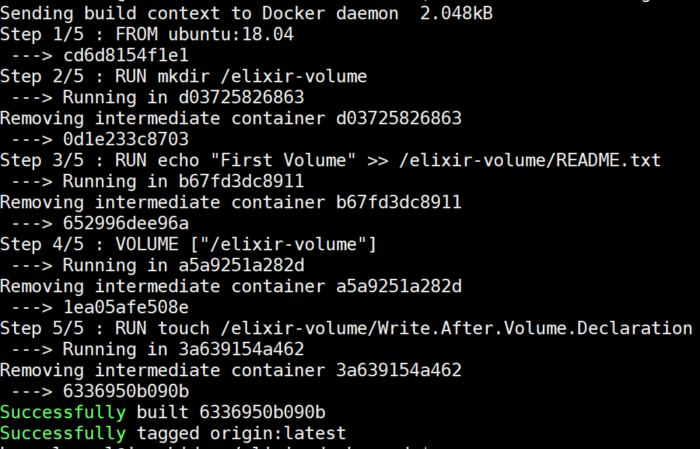
\includegraphics[width=0.8\columnwidth]{./Figure/BuildingDockerfile}
\end{frame}



\frame{
\frametitle {}
\vspace{2cm}
\centerline{\Huge \color{NavyBlue} \textbf{\emph{Dockerfile Best Practices}}}
\vspace{0.5cm}
}

\begin{frame}[fragile]
\frametitle{Dockerfile}
\framesubtitle{from \lstinline!stdin!}

Building an image on the fly, w/o using a static file

\begin{lstlisting}
touch myfile.sh
chmod +x myfile.sh
docker build -t foo . -f-<<EOF
FROM ubuntu:18.04
RUN echo "hello world"
COPY myfile.sh /opt/
EOF
\end{lstlisting}
\end{frame}


\begin{frame}[fragile]
\frametitle{Dockerfile}
\framesubtitle{with a remote context}

\begin{lstlisting}
docker build -t foo \
       https://github.com/thajeztah/pgadmin4-docker.git \
	   -f-<<EOF
	   FROM ubuntu:18.04
	   WORKDIR /usr/local/lib/python2.7/site-packages
	   COPY LICENSE pgadmin4/
	   COPY config_distro.py pgadmin4/
	   EOF
\end{lstlisting}
\end{frame}

\begin{frame}[fragile]
\frametitle{Dockerfile}
\framesubtitle{ignore files}

Unwanted files can be excluded from the context, by convention
a \lstinline!.dockerignore! file is required and using regular expression
is possible to exclude files.
\end{frame}

\begin{frame}[fragile]
\frametitle{Dockerfile}
\framesubtitle{ignore files}

\begin{itemize}
\item \lstinline!#!: defines a comment
\item \lstinline!*/temp*! Exclude files and directories whose names start with temp in any immediate subdirectory of the root.For example, the plain file \lstinline!/somedir/temporary.txt! is excluded, as is the directory \lstinline!/somedir/temp!.
\item \lstinline!|*/*/temp*! Exclude files and directories starting with temp from any sub-directory that is two levels below the root. For example, \lstinline!/somedir/subdir/temporary.txt! is excluded.
\item \lstinline!temp?! Exclude files and directories in the root directory whose names are a one-character extension of temp. For example, \lstinline!/tempa! and \lstinline!/tempb! are excluded.
\end{itemize}
\end{frame}

\begin{frame}[fragile]
\frametitle{Dockerfile}
\framesubtitle{make it human readable}

When possible sorting multi-line arguments is recommended

\begin{lstlisting}
RUN apt-get update &&\
    apt-get install -y \
	    bzr \
		csv \
		git \
		mercurial \
		subversion \
		texlive
\end{lstlisting}
\end{frame}


\begin{frame}[fragile]
\frametitle{Dockerfile}
\framesubtitle{quick tips}

\begin{itemize}
\item Annotate the image with \lstinline!LABEL!
\item Use \lstinline!ENV! for keeping track of versions
\item \lstinline!COPY! is more transparent than \lstinline!ADD!
\item Use \lstinline!wget! or \lstinline!curl! for downloading from the web
\item The web does not guarantee URLs forever
  \begin{itemize}
  \item Consider to host a web/fileserver for \textit{very important} data or software
  \item Licensing can be an issue, some software can not be distributed freely
  \end{itemize}
\item Use \lstinline!WORKDIR! when possible
\item Image as executable ? \lstinline!ENTRYPOINT! is the way to go
  \begin{itemize}
  \item \lstinline!CMD! is used for default parameters \lstinline!--help!
  \end{itemize}
\item A regular user with \lstinline!root! privileges is worst than evil
  \begin{itemize}
  \item This applies only if it is your infrastructure \lstinline!:)!
  \item In most scientific infrastructures Docker is forbidden or masked by some wrapper
  \end{itemize}
\end{itemize}
\end{frame}
 


\frame{
\frametitle {}
\vspace{2cm}
\centerline{\Huge \color{NavyBlue} \textbf{\emph{Private Registry}}}
\vspace{0.5cm}
}


\begin{frame}
\frametitle{Private registry}
A local Docker registry can be useful in many situations
\begin{itemize}
\item images contain private data or information
\item need to test specific applications
\item speed and reliability
\item other applications require the service
\end{itemize}
\end{frame}


\begin{frame}
\frametitle{Private registry}
A local Docker registry can be useful in many situations
\begin{itemize}
\item images contain private data or information
  \begin{itemize}
  \item passwords
  \item user names
  \item network configurations
  \item mount points
  \end{itemize}
\item need to test specific applications
\item speed and reliability
\item other applications require the service
\end{itemize}
\end{frame}


\begin{frame}
\frametitle{Private registry}

A local Docker registry can be useful in many situations

\begin{itemize}
\item images contain private data or information
\item need to test specific applications
\item speed and reliability
  \begin{itemize}
  \item good internet connection
  \item not limited by number of images or containers
  \item lots of disk space
  \end{itemize}
\item other applications require the service
\end{itemize}
\end{frame}


\begin{frame}
\frametitle{Private registry}

A local Docker registry can be useful in many situations

\begin{itemize}
\item images contain private data or information
\item need to test specific applications
\item speed and reliability
\item other applications require the service
  \begin{itemize}
  \item workflow managers may use Docker container for running the pipelines
  \item other container technologies depends on custom Docker images
  \end{itemize}
\end{itemize}
\end{frame}


\begin{frame}[fragile]
\frametitle{Docker Registry}
\framesubtitle{run}
Run an insecure registry

\begin{lstlisting}
$ docker run -d -p 5000:5000 \
           --restart=always \
		   --name registry registry:2
\end{lstlisting}

\textit{!!! WARNING !!!} this is an insecure registry.
\end{frame}

\begin{frame}[fragile]
\frametitle{Docker Registry}
\framesubtitle{run}
Run an insecure registry

\begin{lstlisting}
$ docker run -d -p 5000:5000 \
           --restart=always \
		   --name registry registry:2
\end{lstlisting}

This registry runs on the localhost

and
\end{frame}

\begin{frame}[fragile]
\frametitle{Docker Registry}
\framesubtitle{run}
Run an insecure registry

\begin{lstlisting}
$ docker run -d -p 5000:5000 \
           --restart=always \
		   --name registry registry:2
\end{lstlisting}
This registry runs on the localhost

and

is \textit{INSECURE} but it's OK for testing.
\end{frame}

\begin{frame}[fragile]
\frametitle{Docker Registry}
\framesubtitle{run}

Check if the registry is running

\begin{lstlisting}
$docker ps
CONTAINER ID  IMAGE      COMMAND
d37dd351dd30  registry:2 "/entrypoint.sh /e..."

CREATED    STATUS    PORTS                  
15 min ago Up 15 min 0.0.0.0:5000->5000/tcp 

NAMES
registry
\end{lstlisting}
\end{frame}

\begin{frame}[fragile]
\frametitle{Docker Registry}
\framesubtitle{load an image}

Get an image from the net

\begin{lstlisting}
$ docker pull ubuntu:18.04
\end{lstlisting}
\end{frame}

\begin{frame}[fragile]
\frametitle{Docker Registry}
\framesubtitle{load an image}

Tag the image with a proper name
\begin{lstlisting}
$ docker tag ubuntu:18.04 \
    localhost:5000/user/mydistro:18.04
    
\end{lstlisting}
\end{frame}

\begin{frame}[fragile]
\frametitle{Docker Registry}
\framesubtitle{load an image}

Push the image to the local repository

\begin{lstlisting}
$ docker push \
  localhost:5000/user/mydistro:18.04
\end{lstlisting}
\end{frame}

\begin{frame}[fragile]
\frametitle{Docker Registry}
\framesubtitle{list images}

Docker works with HTTP API (v2)

\begin{lstlisting}
$ curl -v http://localhost:5000/v2/_catalog
\end{lstlisting}

\url{https://docs.docker.com/registry/spec/api/}

\end{frame}

\begin{frame}[fragile]
\frametitle{Docker Registry}
\framesubtitle{list images}

\begin{lstlisting}
< HTTP/1.1 200 OK
< Content-Type: application/json; charset=utf-8
< Docker-Distribution-Api-Version: registry/2.0
< X-Content-Type-Options: nosniff
< Date: Tue, 25 Sep 2018 13:36:04 GMT
< Content-Length: 52
<
{"repositories":["joe/ubuntu","raoul/ubuntu"]}
* Connection #0 to host localhost left intact
\end{lstlisting}
\end{frame}

\begin{frame}[fragile]
\frametitle{Docker Registry}
\framesubtitle{get tags}

\begin{lstlisting}
$ curl http://localhost:5000/raoul/ubuntu/tags/list
{"name":"raoul/ubuntu","tags":["18.04"]}
\end{lstlisting}
\end{frame}

\begin{frame}[fragile]
\frametitle{Docker Registry}
\framesubtitle{get details}

\begin{lstlisting}
$ curl http://localhost:5000/raoul/ubuntu/manifests/18.04
\end{lstlisting}

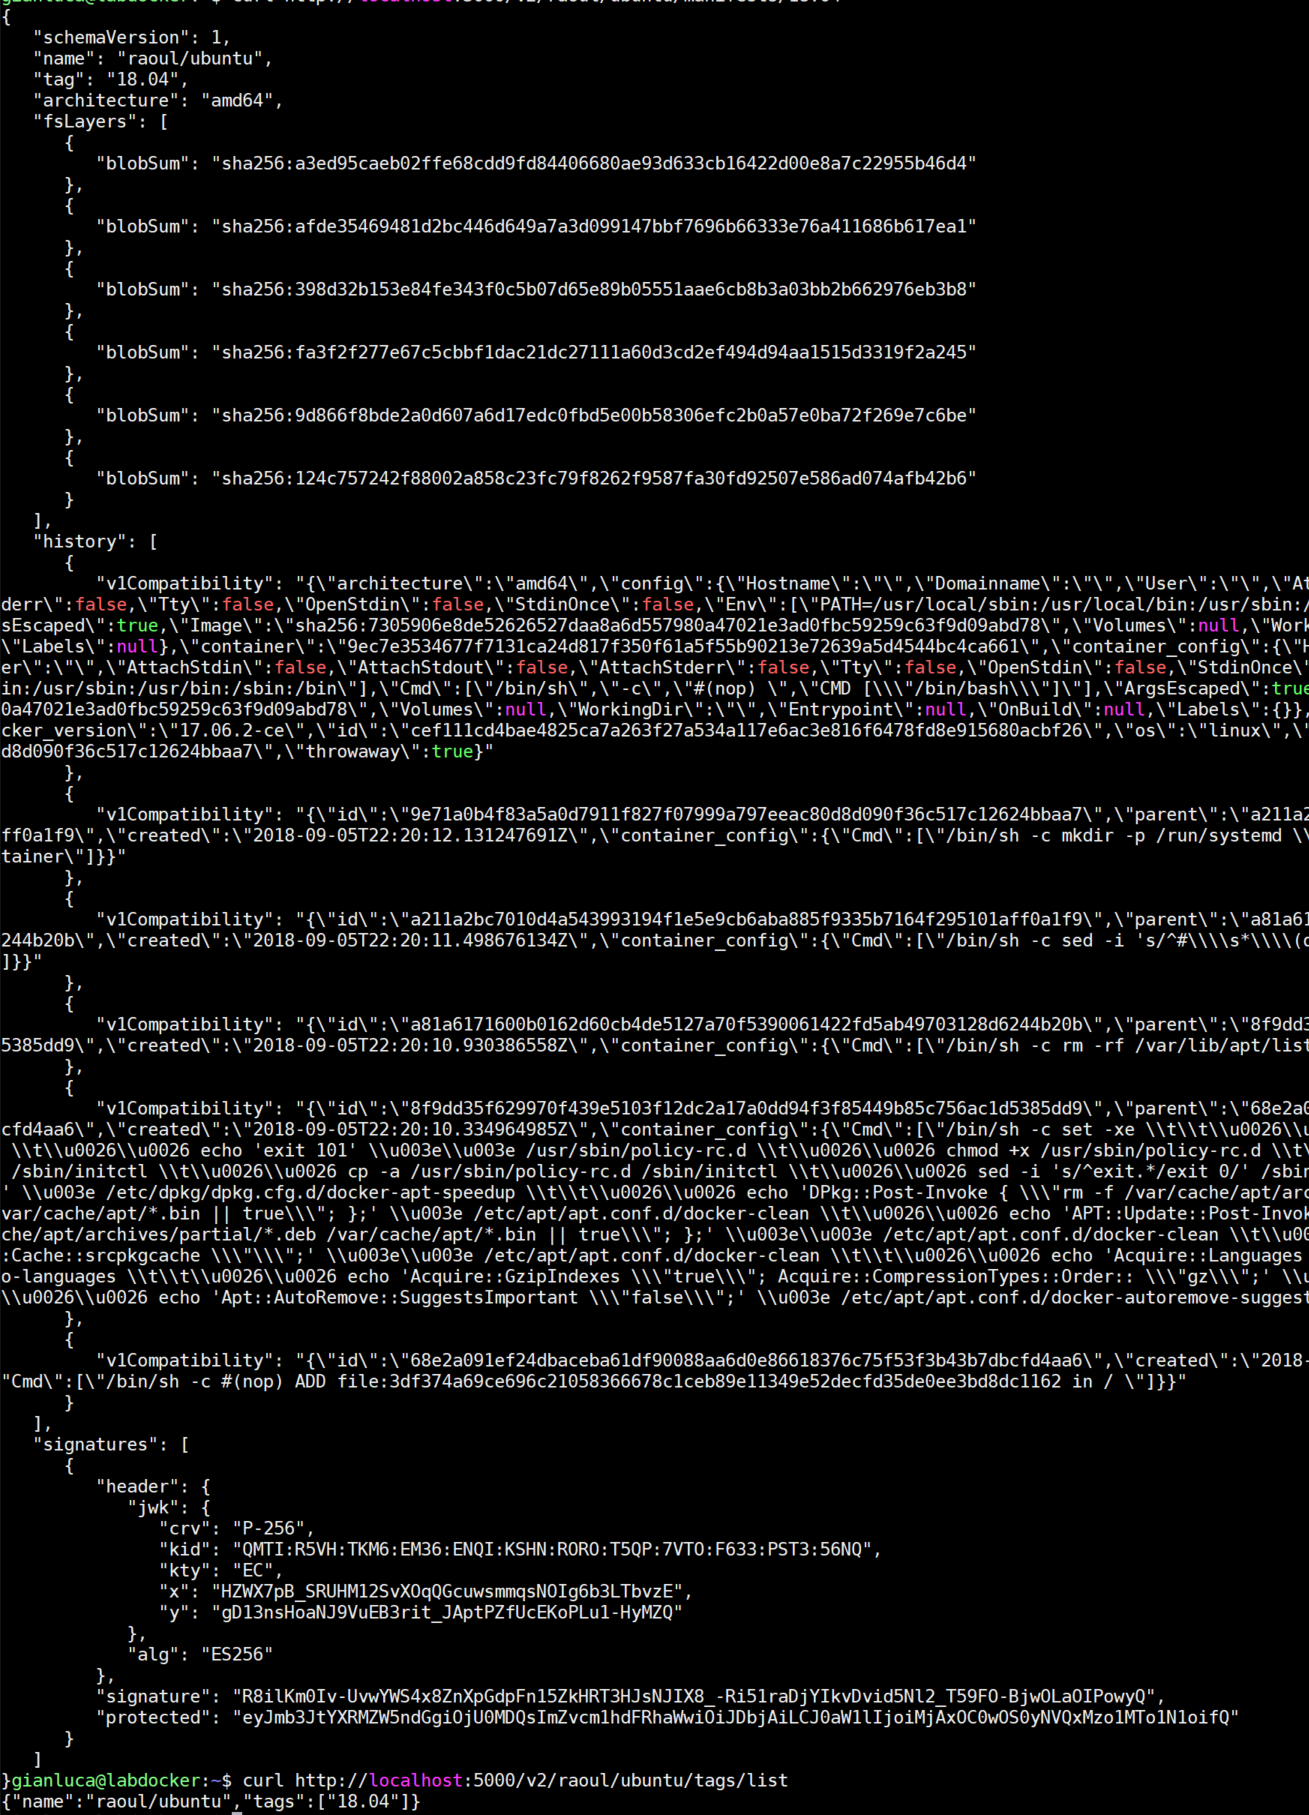
\includegraphics[width=0.8\columnwidth]{./Figure/RegistryDetails}
\end{frame}

\begin{frame}[fragile]
\frametitle{Docker Hub}
\framesubtitle{public registry}

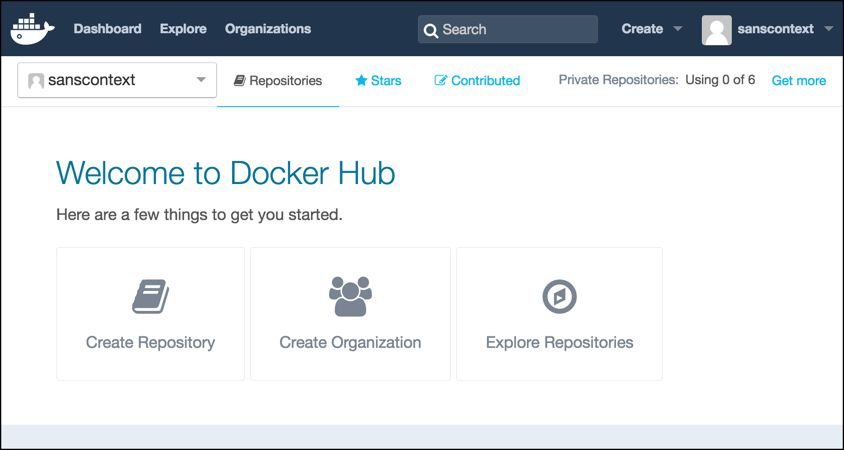
\includegraphics[width=0.8\columnwidth]{./Figure/docker-222-114}
\end{frame}


\begin{frame}[fragile]
\frametitle{Docker Hub}
\framesubtitle{public registry}

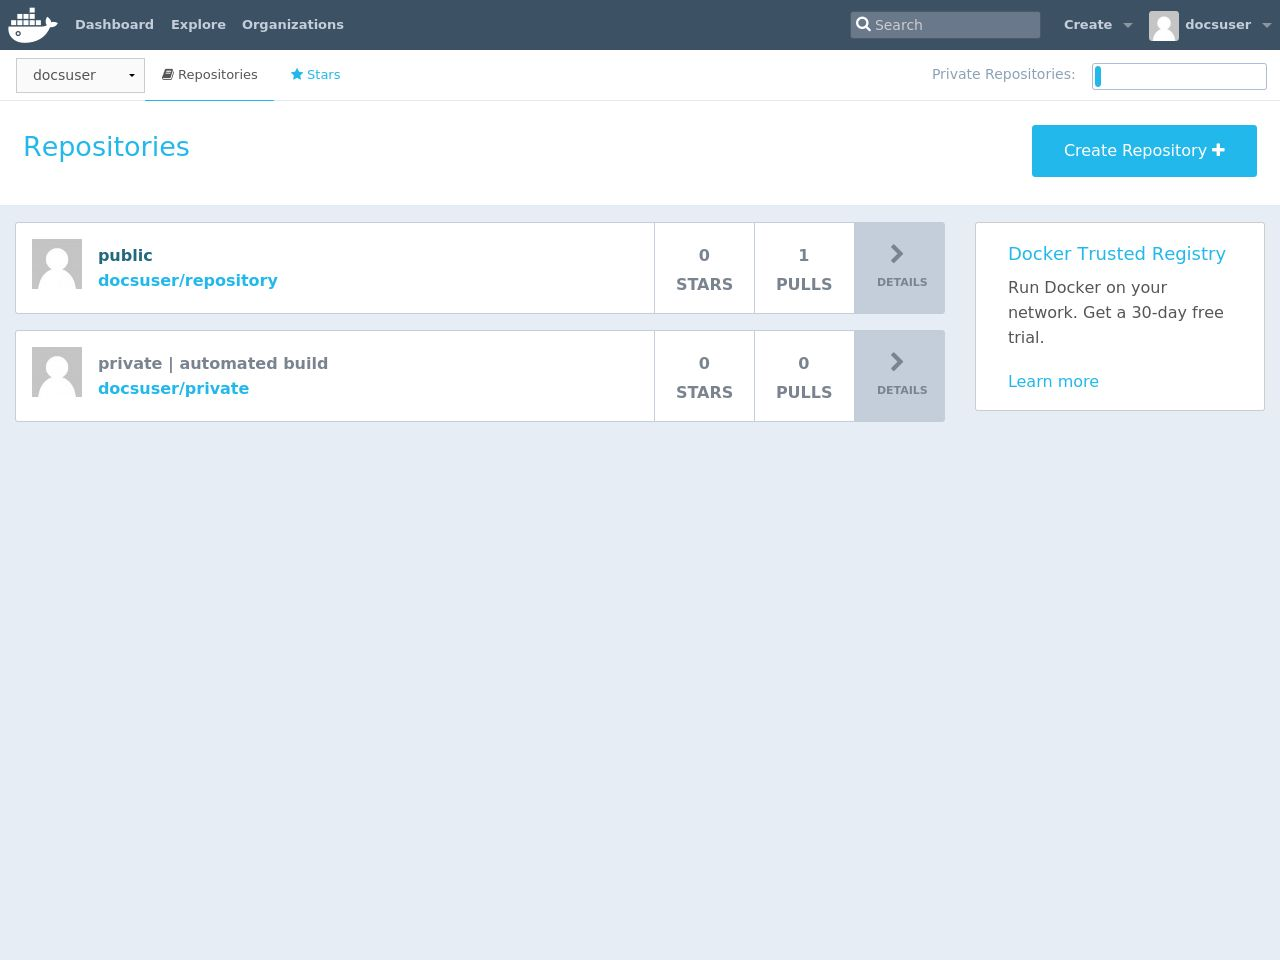
\includegraphics[width=0.8\columnwidth]{./Figure/docker-223-116}
\end{frame}

\begin{frame}[fragile]
\frametitle{Docker Hub}
\framesubtitle{public registry}
\begin{itemize}
\item register a new user to \url{https://hub.docker.com/}
\item \lstinline!export DOCKER_ID_USER="username"!
\item \lstinline!docker login!
\item \lstinline!docker tag imageX $DOCKER_ID_USER/imageX!
\item \lstinline!docker push $DOCKER_ID_USER/imageX!
\end{itemize}
\end{frame}

\frame{
\frametitle {}
\vspace{2cm}
\centerline{\Huge \color{NavyBlue} \textbf{\emph{Swarm}}}
\vspace{0.5cm}
}
\begin{frame}
\frametitle{Swarm}
\framesubtitle{Overview}
Multiple Docker hosts can be managed in a centralized manner using an inner feature of Docker: \textbf{\textit{Swarm}}
\end{frame}

\begin{frame}
\frametitle{Swarm}
\framesubtitle{Overview}
\begin{itemize}
\item Cluster management
\item Decentralized design (one is all)
\item Declarative service model
\item Scaling
\item Desired state reconciliation
\item Multi-host networking
\item Service discovery
\item Load balancing
\item Secure by default (TLS)
\item Rolling updates
\end{itemize}
\end{frame}

\begin{frame}
\frametitle{Swarm}
\framesubtitle{Overview}
A generic Docker Host is a \textit{Node} in the Swarm.
\end{frame}

\begin{frame}
\frametitle{Swarm}
\framesubtitle{Overview}
A generic Docker Host is a \textit{Node} in the Swarm.
\vspace{0.4}
A Node can be:
\begin{itemize}
\item Manger: dispatches task to workers; orchestrate and manage the cluster
\item Worker: executes a task  
\end{itemize}
\end{frame}
   
   \end{document}  

   



